\subsection{Kontrollplatine}
\label{sec:control}
Als Steuerplatine kommt ein FRDM-KL25Z von Freescale zum Einsatz. 
Darauf wird wird ein FRTOS als Betriebssystem eingesetzt. 
Für die Ansteuerung der Peripherie und der externen Komponenten 
werden Komponenten mit Processor Expert erzeugt. 
\begin{figure}[h!]
    \centering
    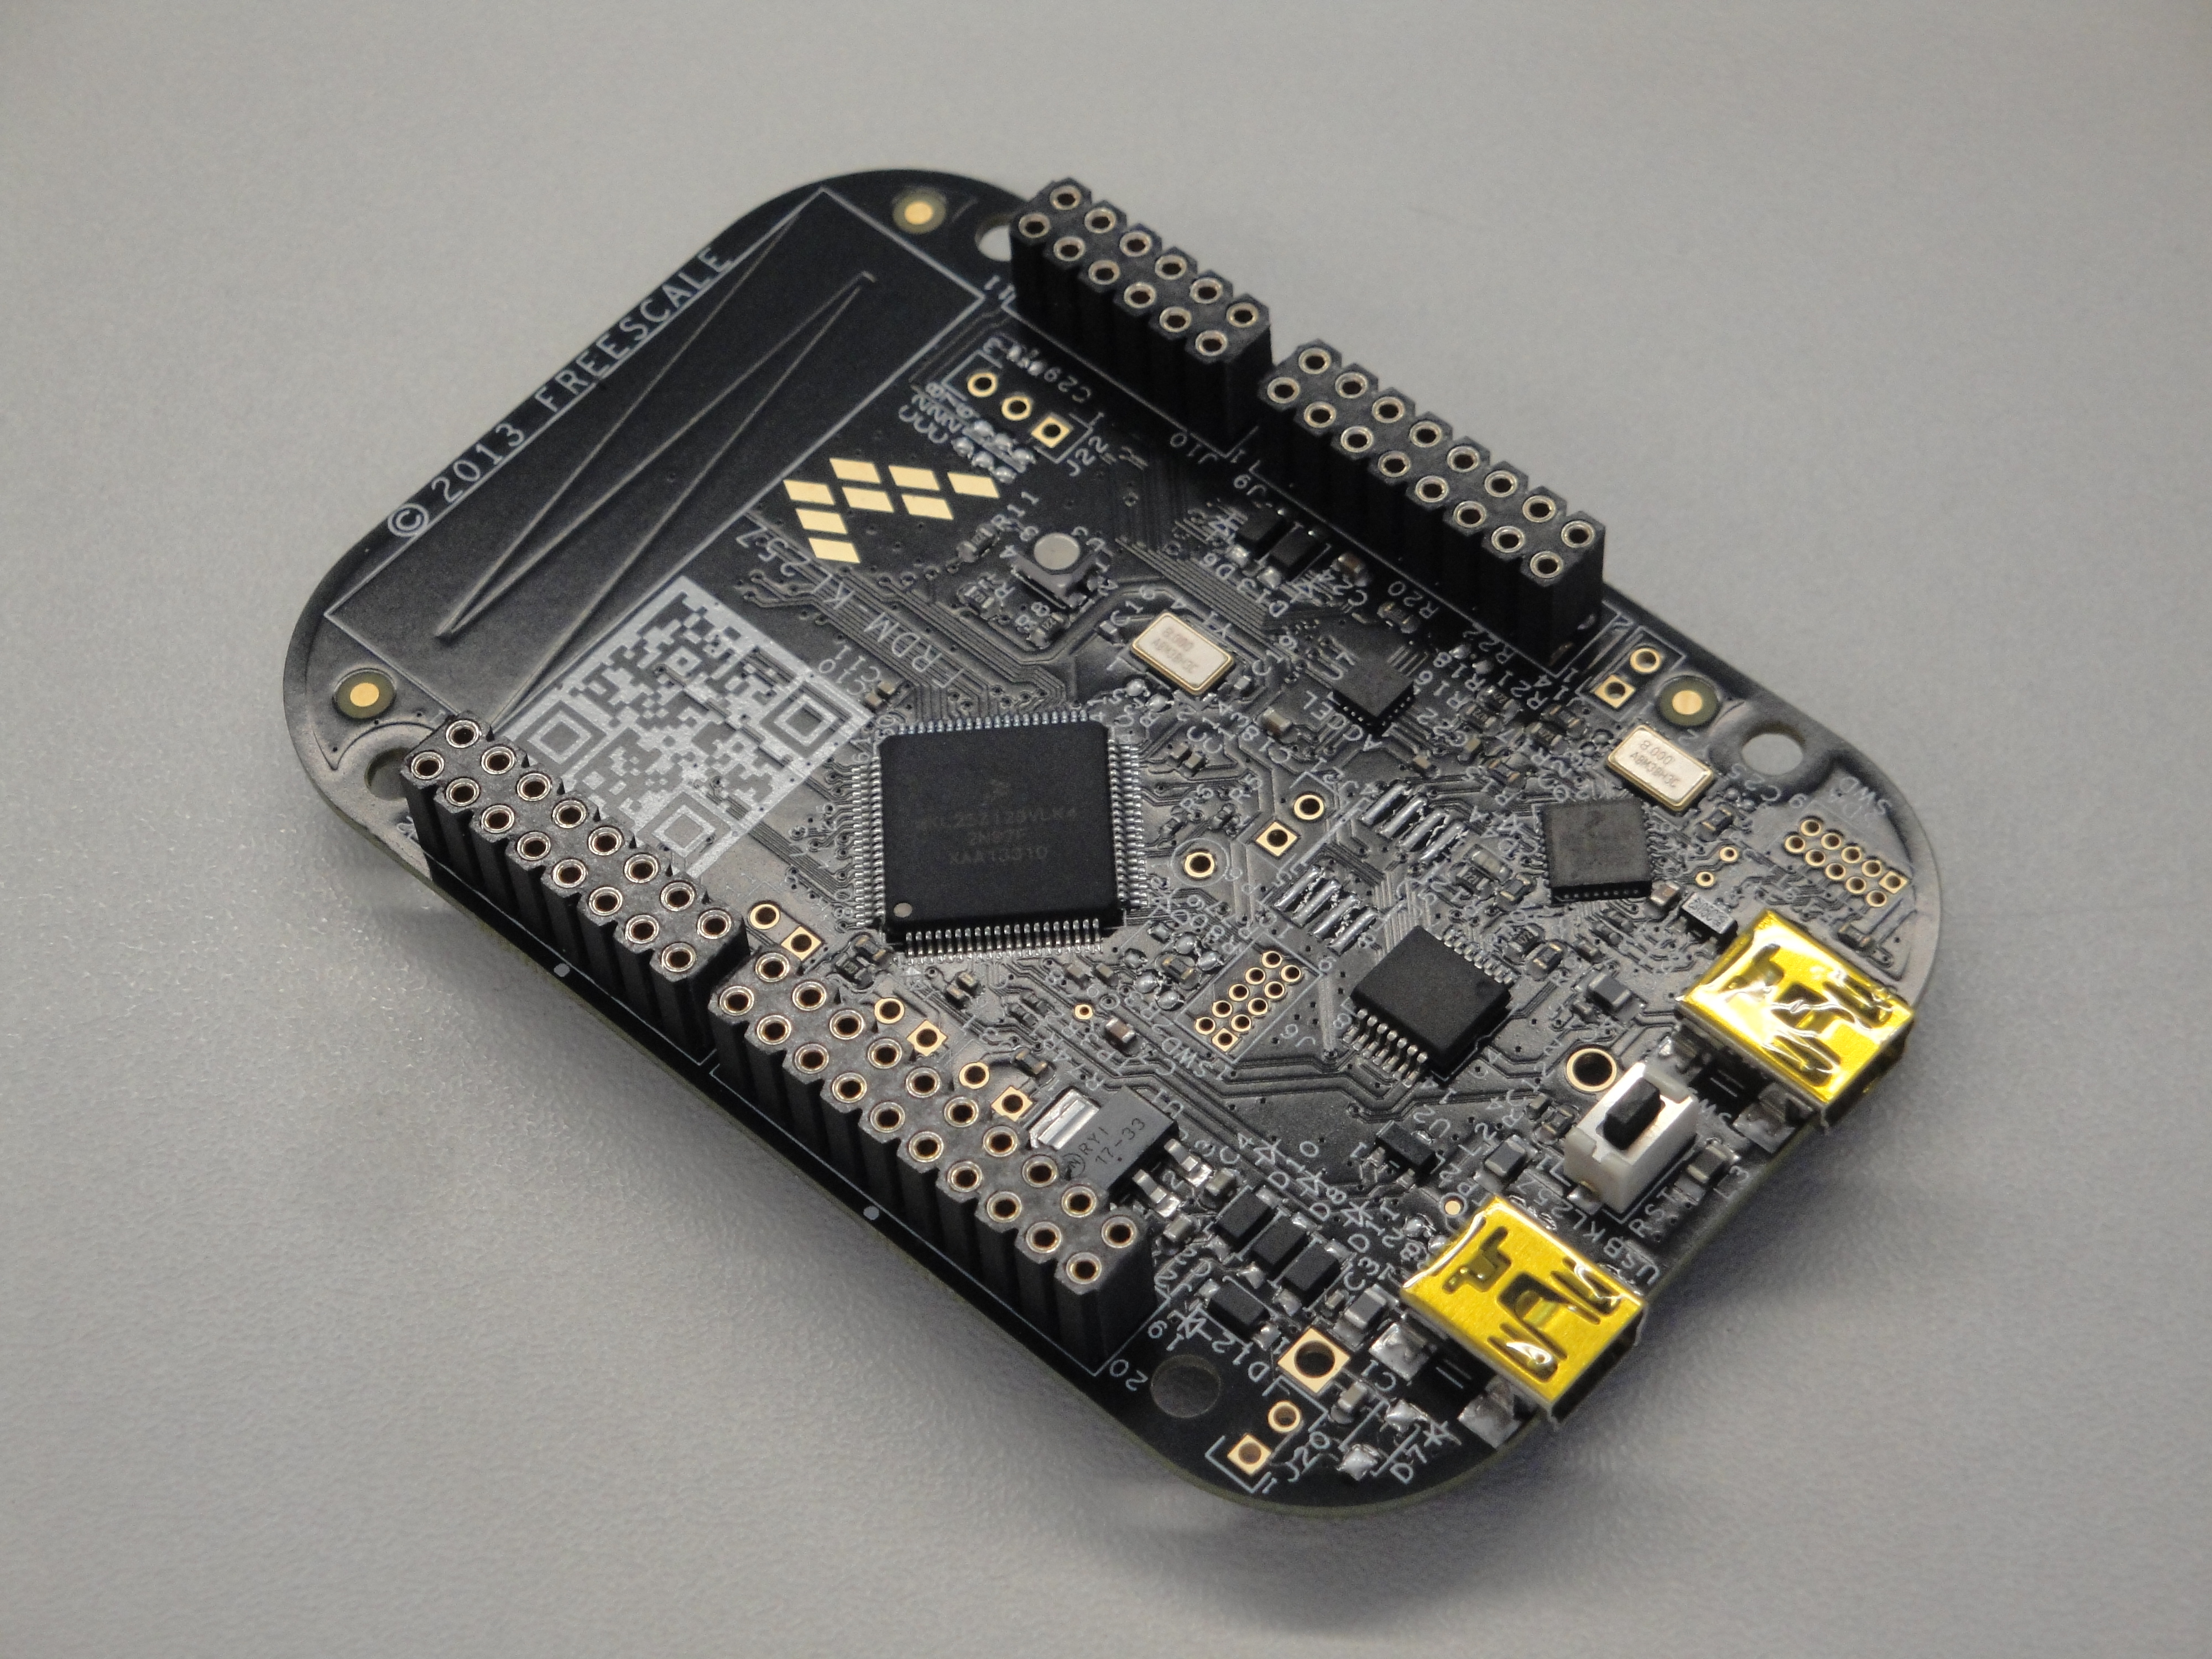
\includegraphics[width=0.7\textwidth]{fig_pcb/DSC02907.JPG}
    \caption{Kontrollplatine - FRDM-KL25Z}
    \label{fig:dc}
\end{figure}
